%%%%%%%%%%%%%%%%%%%%%%%%%%%%%%%%%%%%%%%%%%%%%%%%%%%%%%%%%%%%%%%%%%%%%%%%%%%%%%%%
%%%%%%%%%%%%%%%%%%   Vorlage für eine Abschlussarbeit   %%%%%%%%%%%%%%%%%%%%%%%%
%%%%%%%%%%%%%%%%%%%%%%%%%%%%%%%%%%%%%%%%%%%%%%%%%%%%%%%%%%%%%%%%%%%%%%%%%%%%%%%%

% Erstellt von Maximilian Nöthe, <maximilian.noethe@tu-dortmund.de>
% ausgelegt für lualatex und Biblatex mit biber

% Kompilieren mit
% latexmk --lualatex --output-directory=build thesis.tex
% oder einfach mit:
% make

\documentclass[
  tucolor,       % remove for less green,
  BCOR=12mm,     % 12mm binding corrections, adjust to fit your binding
  parskip=half,  % new paragraphs start with half line vertical space
  open=any,      % chapters start on both odd and even pages
  cleardoublepage=plain,  % no header/footer on blank pages
]{tudothesis}


% Warning, if another latex run is needed
\usepackage[aux]{rerunfilecheck}

% just list chapters and sections in the toc, not subsections or smaller
\setcounter{tocdepth}{1}

%------------------------------------------------------------------------------
%------------------------------ Fonts, Unicode, Language ----------------------
%------------------------------------------------------------------------------
\usepackage{fontspec}
\defaultfontfeatures{Ligatures=TeX}  % -- becomes en-dash etc.

% german language
\usepackage{polyglossia}
\setdefaultlanguage{german}

% for english abstract and english titles in the toc
\setotherlanguages{english}

% intelligent quotation marks, language and nesting sensitive
\usepackage[autostyle]{csquotes}

% microtypographical features, makes the text look nicer on the small scale
\usepackage{microtype}

%------------------------------------------------------------------------------
%------------------------ Math Packages and settings --------------------------
%------------------------------------------------------------------------------

\usepackage{amsmath}
\usepackage{amssymb}
\usepackage{mathtools}

% Enable Unicode-Math and follow the ISO-Standards for typesetting math
\usepackage[
  math-style=ISO,
  bold-style=ISO,
  sans-style=italic,
  nabla=upright,
  partial=upright,
]{unicode-math}
\setmathfont{Latin Modern Math}

% nice, small fracs for the text with \sfrac{}{}
\usepackage{xfrac}


%------------------------------------------------------------------------------
%---------------------------- Numbers and Units -------------------------------
%------------------------------------------------------------------------------

\usepackage[
  locale=DE,
  separate-uncertainty=true,
  per-mode=symbol-or-fraction,
]{siunitx}
\sisetup{math-micro=\text{µ},text-micro=µ}

%------------------------------------------------------------------------------
%-------------------------------- tables  -------------------------------------
%------------------------------------------------------------------------------

\usepackage{booktabs}       % \toprule, \midrule, \bottomrule, etc

%------------------------------------------------------------------------------
%-------------------------------- graphics -------------------------------------
%------------------------------------------------------------------------------

\usepackage{graphicx}
\usepackage{grffile}

% allow figures to be placed in the running text by default:
\usepackage{scrhack}
\usepackage{float}
\floatplacement{figure}{htbp}
\floatplacement{table}{htbp}

% keep figures and tables in the section
\usepackage[section, below]{placeins}


%------------------------------------------------------------------------------
%---------------------- customize list environments ---------------------------
%------------------------------------------------------------------------------

\usepackage{enumitem}

%------------------------------------------------------------------------------
%------------------------------ Bibliographie ---------------------------------
%------------------------------------------------------------------------------

\usepackage[
  backend=biber,   % use modern biber backend
  autolang=hyphen, % load hyphenation rules for if language of bibentry is not
                   % german, has to be loaded with \setotherlanguages
                   % in the references.bib use langid={en} for english sources
]{biblatex}
\addbibresource{references.bib}  % the bib file to use
\DefineBibliographyStrings{german}{andothers = {{et\,al\adddot}}}  % replace u.a. with et al.


% Last packages, do not change order or insert new packages after these ones
\usepackage[pdfusetitle, unicode, linkbordercolor=tugreen]{hyperref}
\usepackage{bookmark}
\usepackage[shortcuts]{extdash}

%------------------------------------------------------------------------------
%-------------------------    Angaben zur Arbeit   ----------------------------
%------------------------------------------------------------------------------

\author{Christopher Krause}
\title{\LaTeX-Dokumentenklasse und Vorlage für Abschlussarbeiten an der TU Dortmund}
\date{2019}
\birthplace{Mainz}
\chair{Lehrstuhl für Experimentelle Physik IV}
\division{Fakultät Physik}
\thesisclass{Bachelor of Science}
\submissiondate{31. September 2015}
\firstcorrector{Prof.~Dr.~Erstgutachter}
\secondcorrector{Prof.~Dr.~Zweitgutachter}

% tu logo on top of the titlepage
\titlehead{\includegraphics[height=1.5cm]{logos/tu-logo.pdf}}

\begin{document}
\frontmatter
\thispagestyle{empty}
\setcounter{page}{2}
\section*{Hinweise}
Empfohlen wird die Verwendung dieser Vorlage mit der jeweils aktuellsten TeXLive Version (Linux, Windows) bzw. MacTeX Version (MacOS).
Aktuell ist dies TeXLive 2016. Download hier:
\begin{center}
  \ttfamily\url{https://www.tug.org/texlive/}
\end{center}
Bei Verwendung von TexLive Versionen 2014 und älter sollte
die Zeile
\begin{center}
\verb+\RequirePackage{fixltx2e}+ 
\end{center}
als erste Zeile der Präambel noch vor der Dokumentenklasse eingefügt werden.
Dies lädt diverse Bugfixes für LaTeX, die ab TexLive 2015 Standard sind.

Die Vorlage \texttt{thesis.tex} ist für die Kompilierung mit \texttt{lualatex} ausgelegt, mit wenigen Anpassungen kann sie aber auch mit \texttt{pdflatex} oder \texttt{xelatex} verwendet werden. 
Die Dokumentenklasse \texttt{tudothesis.cls} kann mit allen drei Programmen verwednet werden.

Achten Sie auch auf die Kodierung der Quelldateien.
Bei Verwendung von Xe\LaTeX\ oder Lua\LaTeX\ (empfohlen) müssen die
Quelldateien UTF-8 kodiert sein.
Bei Verwendung von pdf\LaTeX\ nutzen Sie die Pakete \texttt{inputenc} und \texttt{fontenc} mit der korrekten Wahl der Kodierungen.

Eine aktuelle Version dieser Vorlage steht unter 
\begin{center}
  \ttfamily\url{https://github.com/maxnoe/tudothesis}
\end{center}
zur Verfügung.

Alle verwendeten Pakete werden im \LaTeX{} Kurs von Pep et al.\ erklärt:
\begin{center}
  \ttfamily\url{http://toolbox.pep-dortmund.org/notes}
\end{center}

Für Rückmeldungen und bei Problemen mit der Klasse oder Vorlage, bitte ein \emph{Issue} auf GitHub aufmachen oder eine Email an
\href{mailto:maximilian.noethe@tu-dortmund.de}{maximilian.noethe@tu-dortmund.de} schreiben.

Wenn Sie die Dokumentenklasse mit der Option \texttt{tucolor} laden, werden verschiedene Elemente in TU-Grün gesetzt.

\maketitle

% Gutachterseite
\makecorrectorpage

% hier beginnt der Vorspann, nummeriert in römischen Zahlen
\thispagestyle{plain}

\section*{Kurzfassung}
Hier steht eine Kurzfassung der Arbeit in deutscher Sprache inklusive der Zusammenfassung der
Ergebnisse.
Zusammen mit der englischen Zusammenfassung muss sie auf diese Seite passen.

\section*{Abstract}
\begin{english}
The abstract is a short summary of the thesis in English, together with the German summary it has to fit on this page.
\end{english}

\tableofcontents

\mainmatter
% Hier beginnt der Inhalt mit Seite 1 in arabischen Ziffern
\chapter{Einleitung}
Siliziumdetektoren sind in der Hochenergiephysik und in der Industrie weit verbreitete
Detektoren, welche in Collider-Experimenten, wie Atlas, verwendet werden.
Sie operieren bei Raumtemperatur und können präzise Rückschlüsse auf die
Energie von Teilchen schließen. Einfallende Teilchen können die
Struktur des Detektors verändern, wodurch dieser ineffizienter wird.
Es ist somit notwendig, die Strahlenschäden möglichst gering zu halten damit
die Halbleiter eine möglichst lange Lebenszeit besitzen. Manche Schäden sind durch annealing nicht
aufhebbar, wodurch die Detektoren unweigerlich mit fortlaufendem Einsatz
an Leistungsfähigkeit verlieren. Um die reparablen Schäden im Siliziumkristall
zu beseitigen wird der Annealingeffekt genutzt. Hierbei wird durch zugeführte Wärme gewisse
Defekte entfernt.
Zusätzlich sorgt die Bestrahlung der Detekoren für einen anwachsenden Leckstrom, welcher den
gemessenen elektrischen Signalen überlagert ist und ein Rauschen kreiert. Ein
effektiver Detektor sollte somit einen möglichst geringen Leckstrom haben.
Für einen Detektor ist eine möglichst große Depletionszone ebenfalls wichtig, idealerweise
liegt eine vollständige Depletion des Detekorvolumens vor. Um dies zu erreichen wird
eine externe Spannung verwendet. Mit steigender Spannung wächst jedoch auch der Leckstrom, weshalb
darauf geachtet werden muss bei möglichst geringer externer Spannung den Detektor zu depletieren.
Dies ist abhängig von der Dotierungskonzentration, da sie die Ladung der
Raumladungszone beschreibt.

Die durch Strahlung induzierte Änderung der Dotierungskonzentration und des Leckstromes sind
somit wichtige Größen für die Qualität eines Detektors. In dieser Arbeit wird das
theoretische Verhalten der beiden Größen auf der Grundlage des Hamburger-Modells betrachtet.
Ein Programm zur Modellierung von Annealingeffekten kann somit zur
optimierung des Annealingprozesses beitragen.


Das oben erwähnte Collider-Experiment, ATLAS, verwendet Siliziumdetekoren als
einen Teil seines inneren Detektors zur Bestimmung von Richtung, Impuls
und Ladung von geladenen Teilchen. Es ist Teil des LHC am Cern und umfasst
das größte Volumen aller Detektoren, die bisher gebaut wurden\cite{atlas}.
Der innere Detektor ist zylinderförmig mit einer Länge von $\SI{6.2}{\meter}$ und
einem Radius von $\SI{2.1}{\meter}$. Er wird von einem $\SI{2}{\tesla}$ Magnetfeld
durchsetzt und kann Teilchen mit geringen Energien von $\SI{0.5}{\giga\eV}$ noch detektieren.
Bestehend aus drei Komponenenten, dem Pixeldetektor, dem "Semiconductor Tracker" (SCT) und dem "Transition Radiation Tracker" (TCT) kommen  die
Siliziumdetektoren in allen drei Bestandteilen zum Einsatz.
Mit einer Fläche von $\SI{1.7}{\meter\squared}$, drei Lagen und insgesamt 1744 Modulen ist es möglich
Information über die Strecke der entstehenden Teilchen zu erlangen. Der SCT besteht aus 4088 Modulen über vier zylindrische Lagen,
sowie 18 scheibenförmige Lagen, verteilt und umfasst eine Fläche von $\SI{63}{\meter\squared}$. Auch dieser wird für
die Rekonstruktion der Bahn der Teilchen verwendet, jedoch auch für die Identifikation und der Bestimmung des Impulses der Teilchen.
Der TCT wird ebenfalls zur Identifikation von Teilchen, hauptsächlich Elektronen und Pionen, verwendet und besteht aus 73 Lagen
von Straw-Detektoren (viele aneinander gereihte Proportionalzählrohre).

\chapter{Theoretische Grundlagen}


\section{Siliziumhalbleiterdetektoren}

Die Siliziumhalbleiter sind in der hochenenergie Physik weit verbreitete
Detektoren, welche in Collider-Experimenten , wie Atlas, verwendet werden.
Sie operieren bei Raumtemperatur und können präzise Rückschlüsse auf die
Energie von Teilchen schließen.


Die im Halbleiter vorkommenden Elektronen des Siliziumkristalls wechselwirken mit anderen Elektronen und
Kernen, wodurch es zu vielen Aufspaltungen des Energieniveaus dieser kommt. Die
Zustände liegen dicht bei einander, weshalb von Energiebändern gesprochen wird.
Das höchste von den Elektronen besetzte Band ist das Valenzband, welches von dem
nächsthöheren Band durch eine Bandlücke getrennt ist. Elektronen können
durch Anregungen in das Leitungsband wandern und somit Strom leiten, vorrausgesetzt
die Anregungen sind größer als die Energielücke.

Das Einbringen von Fremdatomen in den Siliziumkristall kann dessen Eigenschaften ändern
und wird Dotierung genannt.
Hat das Fremdatom mehr oder weniger Valenzelektronen als das Silizium, kommt
es zu weiteren Aufspaltungen der Energieniveaus, welche sich in der Energielücke
befindet. Dadurch wird es für Elektronen einfacher in das Leitungsband zu wandern.
Bei den Fremdatomen wird zwischen Donatoren und Akzeptoren unterschieden, wobei die
Ersteren mehr Valenzelektronen als das Silizium besitzen und die Zweiteren weniger.
Bereiche des Siliziumkristalls mit Donatoren werden n-Dotierte Halbleiter
und Bereiche mit Akzeptoren p-Dotierte Halbleiter genannt.

Bei einem Übergang von einer n-Dotierten zu einer p-Dotierten Schicht rekombinieren
die Elektronen der n-Dotierten Schicht mit den Elektronenlöchern der p-dotierten Schicht, da beide
in die anderen Bereiche diffundieren. Durch die übrig bleibenden Ortsfesten Atomkerne
baut sich ein elektrisches Feld auf, welches dem Diffusionsstrom entgegen wirkt.
Ein sich einstellendes Gleichgewicht führt zu einer raumladungsfreien Zone bei
dem p-n-Übergang.
Durch eine äußere Spannung wird die Zone vergrößert und dient als Ionisationskammer für einfallende Teilchen.
Die entstehenden Elektronen-Loch Paare werden als elektrisches Signal gemessen.


\section{Strahlenschäden}
Wechselwirkungen von hochenergetischen Teilchen mit Siliziumhalbleitern können zu Defekten in deren
Gitterstruktur führen.
Die Energie der Teilchen an die Gitteratome wird dabei durch Ionisation und elastischer Streuung abgegen.
Es muss zwischen verschiedenen Arten von Defekten unterschieden werden. Die Teilchen können ein Gitteratom aus dem
Gitter herausschlagen, wodurch eine Leerstelle und ein Zwischengitteratom entsteht. Das herausgeschlagene Atom
kann Silizium, aber auch ein Fremdatom sein. Daraus folgt eine Änderung der Dotierungskonzentration im
Halbleiter und somit eine Änderung seiner Eigenschaften.

Um Fluenzen $ \Phi$ von verschiedenen Teilchen (Lepton, Hadron, Photon) miteinander vergleichen zu können, werden diese
auf eine $1$MeV Neutronstrahlung normalisiert und haben die Einheit $\mathrm{\frac{n_{\mathrm{eq}}}{cm^2}}$.


\section{Annealing}
Annealing beschreibt allgemein die durch Erhitzung hervorgerufenen Veränderungen von Materialeigenschaften. Für die
Siliziumhalbleiter sollen dabei, durch die zugeführte Wärme, die Defekte teilweise behoben werden um somit eine
bessere Funktionsfähigkeit über einen längeren Zeitraum zu garantieren. Die auftetenden Effekte sind dabei wie folgt:

\textbf{1. Migration:} Ist die Temperatur hoch genug können die Zwischengitteratome durch das Gitterwandern und
zum einen Leerstellen im Gitter füllen.

\textbf{2. Komplexformation:} Das migrieren der Atome kann zum Ausbilden von Komplexen führen. So kann sich zum Beispiel ein
Zwischengittersiliziumatom mit einem Siliziumatom im Gitter binden.

\textbf{3. Dissoziation:} Komplexe können bei hohen Temperaturen Dissoziieren, wodurch einzelne Bestandteile des Komplexes
durch das Gitter migrieren können. Dafür muss die Schwingungsenergie des Gitters größer als die Bindungsenergie der Komplexe sein.

Die Annealingeffekte bewirken eine Änderung in der Dotierungskonzentration $N_{\mathrm{eff}}= |N_{\mathrm{D}}-N_{\mathrm{A}}|$, welches durch das Hamburger Modell beschrieben wird.
Die Änderung von $N_{\mathrm{eff}}$ ist gegeben durch:
\begin{align}
  \Delta N_{\mathrm{eff}}(t, \Phi_{\mathrm{eq}}, T)   = N_{\mathrm{C}}(\Phi_{\mathrm{eq}}) + N_{\mathrm{A}}(t, \Phi_{\mathrm{eq}}, T) + N_{\mathrm{Y}}(t, \Phi_{\mathrm{eq}}, T)
\end{align}
Die einzelnen Summanden werden im folgenden erläutert.

\textbf{\textit{Stable Damage}} $\symbf{N_{\mathrm{C}}}:$ Der stable Damage ist unabhängig von der Temperatur und wird durch das annealing nicht beeinflusst.
\begin{align}
  N_{\mathrm{C}}(\Phi_{\mathrm{eq}}) = N_{\mathrm{C0}}[1-\exp{(-c \cdot \Phi_{\mathrm{eq}})}] + g_{\mathrm{c}} \cdot \Phi_{\mathrm{eq}}
\end{align}
Der erste Summand folgt aus einer unvollständigen Entfernung von Donatoren, der zweite Summand beschreibt stabile Defekte, welche sich wie Akzeptorenverhalten \cite{beyer}.


\textbf{\textit{Shortterm annealing}} $\symbf{N_{\mathrm{A}}}:$ Das shortterm annealing bewirkt eine Verringerung der Dotierungskonzentration und entsteht durch
das Annealing von Akzeptoren, was zu einer kleineren Dotierungskonzentration führt. . Dieser Effekt soll
zur Ausheilung des Sensors verwendet werden. Die Bezeichnung rührt daher, dass $N_{\mathrm{A}}$ meistens in den ersten 100 Minuten verschwindend gering wird. Die
Funktion wird näherungsweise beschrieben durch:
\begin{align}
  N_{\mathrm{A}}(t, \Phi_{\mathrm{eq}}, T) = \Phi_{\mathrm{eq}} \cdot g_{\mathrm{a}} \cdot \exp{\left(-\frac{t}{\tau_{\mathrm{a}}}\right)}
\end{align}


\textbf{\textit{Longterm annealing}} $\symbf{N_{\mathrm{A}}}:$

\chapter{Wichtige Hinweise zum Dokument}\label{make}

Diese Vorlage ist auf die Kompilierung mit \texttt{lualatex} ausgelegt. 
Als Dokumentenklasse  wird die \KOMAScript\-Klasse \texttt{scrbook} verwendet.
Falls Sie Änderungen am Layout vornehmen möchten, lesen Sie die \KOMAScript-Dokumentation: \cite{koma}.

Eine umfangreiche Einführung in die moderne Verwendung von \LaTeX{} gibt es hier: \cite{toolbox}, lesenswert ist außerdem das \LaTeX-Tabu: \cite{l2tabu}

Um dieses Dokument vollständig zu erstellen sind maximal vier Programmläufe nötig:
\begin{enumerate}[nosep]
    \item \texttt{lualatex BachelorArbeit.tex}
    \item \texttt{biber BachelorArbeit.bcf}
    \item \texttt{lualatex BachelorArbeit.tex}
    \item \texttt{lualatex BachelorArbeit.tex}
\end{enumerate}

Beim ersten Lauf des \LaTeX-Compilers werden die Kapitel, Links und zitierten Bibliographieeinträge in Hilfsdateien geschrieben.

Dann ist ein Lauf des Programms \texttt{biber} nötig, welches die benötigten Einträge aus der Hilfsdatei einliest, die Einträge aus der \texttt{.bib} Datei einliest, sortiert und formatiert und in eine weitere Hilfsdatei schreibt.

Beim nächsten \LaTeX-Lauf werden dann diese Hilfsdateien eingelesen und Literatur- und Inhaltsverzeichnis erstellt.

Manchmal ist ein vierter Lauf nötig, falls sich durch das einfügen des Literaturverzeichnisses Seitenzahlen verändert haben.

Das Tool \texttt{latexmk} übernimmt dies mit nur einem Programmaufruf und
führ nur so viele Aufrufe durch, wie nötig sind.

\texttt{latexmk --lualatex BachelorArbeit.tex}

Eine gute Option ist es, den \LaTeX{} Output in einem anderen 
Ordner zu erzeugen, dies ist mit der \texttt{--output-directory} Option möglich:

\texttt{latexmk --output-directory=build --lualatex BachelorArbeit.tex}


\section{Erstellen des Ausgabedokuments mit Make}

Für diese Vorlage wird ein Makefile zur Verfügung gestellt, welches automatisch alle Schritte ausführt, die für das fertige Dokument nötig sind.
Die Ausgabe erfolgt dabei in den Unterordner \texttt{build/}.
Make prüft, ob die Quelldateien verändert wurden, falls nicht, werden auch keine Befehle ausgeführt.

Falls Sie das Makefile benutzen möchten, sollten Sie alle Abhängigkeiten eintragen (Eigene Dateien für Kapitel, Plots, etc.).


Download und weitere Informationen zu Make gibt es unter \cite{make}. Die Befehle sind für die Bash ausgelegt.
Wenn Sie sie unter Windows nutzen wollen, benötigen Sie einen Bash-Emulator, wie Git Bash, Download unter \cite{gitbash} möglich.
Wenn Sie Make installiert haben, rufen Sie einfach in der Konsole im Verzeichnis der Arbeit den Befehl \texttt{make}.

\section{Erstellen des Ausgabedokuments mit Texmaker}
\subsection{Einrichten der nötigen Befehle}
Ein beliebter Editor für alle Betriebssysteme ist Texmaker, Download unter \cite{texmaker}.
Damit Texmaker das Dokument korrekt kompiliert, fügen sie einen benutzerdefinierten Befehl hinzu:
\begin{enumerate}[nosep]
    \item Klicken sie oben in der Menüleiste auf \emph{Benutzer/in}
    \item Klick auf \emph{Eigene Befehle}
    \item Klich auf \emph{Eigene Befehle editieren}, dort können Sie bis zu 5 eigene Befehle definieren
    \item Geben Sie dem Befehl unter \emph{Menüeintrag} einen Namen und tragen sie folgende Befehle in das Befehlsfeld ein: \\
      \small\verb+latexmk --lualatex --interaction=batchmode --halt-on-error %.tex |+
    \item Bestätigen Sie mit \emph{OK}
\end{enumerate}

\begin{figure}
    \centering
    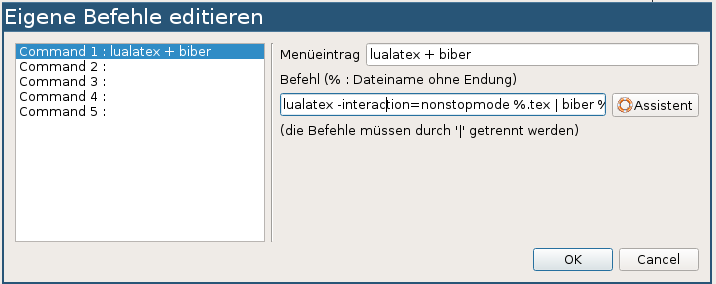
\includegraphics[width=12cm]{Plots/texmaker.png}
    \caption{Screenshot zur Erstellung des Kompilier-Befehls in Texmaker}
    \label{fig:texmaker}
\end{figure}


In Abbildung \ref{fig:texmaker} ist ein Screenshot des Befehlsmenü gezeigt. Ihren Befehl können Sie nun im Drop-Down-Menü zum 
Kompilieren des Dokuments auswählen und mit einem Klick auf den Pfeil starten.

\subsection{Aufräumen}

Nach einem \LaTeX-Fehler ist es oft notwendig, die erstellten Hilfsdateien zu löschen.
Klicken Sie hierzu auf \emph{Werkzeuge}→\emph{Aufräumen}.


\chapter{\LaTeX-Grundlagen}

Bitte beachten Sie beim Schreiben der Arbeit folgende Konventionen bzw. Grundlagen:

\begin{itemize}
    \item \textbf{Abschnitte und Zeilenumbrüche} \\
        Es sollten im Fließtext keine Zeilenumbrüche mit \textbackslash\textbackslash \ erzwungen werden.
        Schreiben Sie höchsten einen Satz in eine Code-Zeile.
        Absätze werden im Code mit einer Leerzeile markiert und dann entsprechend der Einstellung von \texttt{parskip} in der Dokumentenklasse gesetzt.
    \item \textbf{Kursiv/Aufrecht} \\
        \begin{itemize}
            \item Variablen und physikalische Größen werden kursiv gesetzt. 
            \item Einheiten werden immer aufrecht und mit einem halben Leerzeichen Abstand zur Zahl gesetzt. Nutzen Sie \texttt{siunitx}!
            \item Mathematische Konstanten und Funktionen werden ebenfalls aufrecht gesetzt. Zum Beispiel die Eulersche Zahl e, das imaginäre i und das infinitesimale d.
                Im Mathematikmodus können Sie dies mit dem Befehl \verb_\mathrm{}_ erreichen. Für die Funktionen stellt \LaTeX \ Befehle bereit, z.B. \verb+\arccos+.
            \item Integrand und ein $\mathrm{d}x$ sollten ebenfalls durch ein kleines Leerzeichen (\verb+\,+) getrennt werden.
        \end{itemize}
        


\end{itemize}

\section{Zahlen und Einheiten}

Jede Zahl, jede Einheit und jede Zahl mit Einheit sollte mit Hilfe der in dem Paket \texttt{siunitx} zur Verfügung gestellten Befehle gesetzt werden.
Grundsätzlich gilt: Einheiten werden aufrecht gesetzt und haben ein kleines Leerzeichen (\verb+\,+) Abstand zu ihrer Zahl. 
Werden Fließkommazahlen ohne \texttt{siunitx} gesetzt, entsteht ein hässlicher Leerraum zwischen Komma und erster Nachkommastelle, da \LaTeX \ das Komma nicht als Dezimaltrennzeichen, sondern als Satzzeichen interpretiert.

Das Paket wurde mit deutschen Spracheinstellungen (also mit Komma als Dezimaltrennzeichen und $\cdot$ zwischen Zahl und Zehnerpotenz) geladen, sowie mit den Einstellungen, dass die Standardabweichung stets durch $\pm$ abgetrennt wird und Einheiten falls nötig als Brüche ausgegeben werden.

\begin{table}
    \centering
    \caption{Beispiele für siunitx}
    \label{tab:si}
    \begin{tabular}{l r}
        \toprule
        Befehl     &   Ergebnis \\
        \midrule
        \verb+\num{1.2345}+ & \num{1.2345} \\
        \verb+\num{1.2e3}+ & \num{1.2e3} \\
        \verb_\num{1.2 +- 0.2}_ & \num{1.2+-0.2} \\
        \verb+\num{10000}+ & \num{10000} \\
        \verb+\si{\meter\per\second}+ & \si{\meter\per\second} \\
        \verb+\SI{1.2(1)}{\micro\ampere}+ & \SI{1.2(1)}{\micro\ampere} \\
        \verb+\SI{1.2\pm0.1e3}{\kilo\gram\per\cubic\meter}+ & \SI{1.2\pm0.1e3}{\kilo\gram\per\cubic\meter} \\
        \bottomrule 
    \end{tabular}
\end{table}

Das Paket stellt unter anderem die drei wichtigen Befehle
\begin{itemize}
    \item \texttt{\textbackslash num\{Zahl\}},
    \item \texttt{\textbackslash si\{Einheit\}} und
    \item \texttt{\textbackslash SI\{Zahl\}\{Einheit\}}
\end{itemize}
zur Verfügung.
Diese Befehle sollten stets genutzt werden, wenn Zahlen angegeben werden. 
Sie funktionieren sowohl im Text- als auch im Mathematikmodus.
In Tabelle \ref{tab:si} sind einige Beispiele aufgetragen. Bitte lesen Sie die Dokumentation \cite{siunitx}.

\section{Das Literaturverzeichnis}

Das Literaturverzeichnis wird mit Hilfe von BibLaTeX und biber erstellt.
Tragen Sie alle ihre Quellen in die Datei \texttt{references.bib} ein, Sie enthält bereits
einige Beispiele. Für weitere Informationen lesen Sie bitte die Dokumentation \cite{biblatex}.

Im Text können Sie mit \verb_\cite{kürzel}_ zitieren. Seitenzahlen geben Sie in eckigen Klammern an:
\verb_\cite[10]{kürzel}_. 

Das Literaturverzeichnis ist so eingestellt, dass es Ihre Quellen in alphabetischer Reihenfolge nach Autoren nummeriert.
Möchten Sie das Literaturverzeichnis nach der Reihenfolge des Auftauchens im Text sortieren, fügen sie die Paktetoption \texttt{sorting=none} beim Laden
des BibLaTeX-Pakets hinzu.

Den Zitier- und Bibliographie-Stil geben sie mit der Option \texttt{style=Stil} an. Die beiden gebräuchlisten Stile sind \texttt{numeric} und \texttt{alphabetic}. 
Bei \texttt{numeric} werden die Quellen durchnummeriert, bei \texttt{alphabetic} wird ein Buchstabenkürzel aus Autor(en)-Name(n) und Jahr verwendet.
Für weitere Stile konsultieren Sie bitte die Dokumentation: \cite{biblatex}.

Ein Beispiel für das Zitieren eines Buches lautet so \cite{handbook_adhesives},
wissenschaftliche Artikel hingegen werden so \cite{einstein} zitiert.

Damit das Literaturverzeichnis erstellt wird, ist ein Aufruf von \texttt{biber} nach einem ersten kompilieren mit \texttt{lualatex} nötig.
Danach muss das Dokument erneut mit \texttt{lualatex} kompiliert werden. 

Zum korrekten Kompilieren des Dokuments siehe Kapitel \ref{make}.

\chapter{Abbildungen und Tabellen}

\section{Abbildungen}

Achten Sie bei ihren Plots auf ausreichend große Achsenbschriftungen, ausreichende Schriftdicken und gut unterscheidbare Farben.
Im Idealfall haben Sie im Plot und der Arbeit die gleiche Schriftgröße und Schriftart.
Dies lässt sich durch Erstellen des Plots in der korrekten Größe und Einbinden mit dem optionalen Argument \texttt{scale=1} erreichen. Ein Beispiel sehen Sie in Abbildung \ref{fig:bsp}.

Nutzen Sie wenn möglich Vektorgrafiken (pdf) und nur in Ausnahmen Rastergrafiken wie .png oder .jpg.
Setzen Sie Punkte hinter Abbildungsunterschriften.

\begin{figure}
    \centering
    \includegraphics[scale=1]{./Plots/Histogramm.pdf}
    \caption{Ein Histogramm mit Fehlerbalken für zwei Datensätze, Schriftgröße und -art entsprechen der des Dokuments.}
    \label{fig:bsp}
\end{figure}

\section{Tabellen}

Tabellen sollten so einfach wie möglich aufgebaut sein, verzichten Sie auf zu viele Linien. In fast allen Fällen reichen drei horizontale Linien aus, jeweils über und unter der Tabelle und zwischen den Spaltenüberschriften und der eigentlichen Tabelle.

Das Paket \texttt{booktabs} stellt hierfür \verb_\toprule_, \verb_\midrule_ und 
\verb_\bottomrule_ zur Verfügung.
Das Paket \texttt{siunitx} stellt eine extrem mächtige neue Spalteneinstellung bereit: \texttt{S}, mit ihr können Zahlen und Einheiten sehr sauber und gut ausgerichtet gesetzt werden.

Diese Vorlage geht von Tabellenüberschriften aus, möchten Sie dagegen Tabellenunterschriften entfernen Sie das entsprechende optionale Argument für die Dokumentenklasse in der Präambel.

Ein Beispiel ist Tabelle~\ref{tab:bsp}.
\begin{table}
    \centering
    \caption{Beispieltabelle mit willkürlichen Werten, für die Zahlenwerte wurde die S-Option aus \texttt{siunitx} verwendet.}
    \label{tab:bsp}
    \begin{tabular}{S[table-format=4.2] S[table-format=3.2]}
        \toprule
        {$p \mathrel{/} \si{\pascal}$}  & {$T \mathrel{/} \si{\kelvin}$} \\
        \midrule
        1024,23 & 273,15 \\
        1025,31 & 274,5 \\
        1026,27 & 276,2 \\
        \bottomrule
    \end{tabular}
\end{table}


\appendix
% Hier beginnt der Anhang, nummeriert in lateinischen Buchstaben
\chapter{Ein Anhangskapitel}

Hier könnte ein Anhang stehen, falls Sie z.\,B.\ Code, Konstruktionszeichnungen oder Ähnliches mit in die Arbeit bringen wollen.
Im Normalfall stehen jedoch alle Ihre Resultate im Hauptteil der Bachelorarbeit und ein Anhang ist überflüssig.


\backmatter
\printbibliography

\cleardoublepage
\thispagestyle{empty}
\section*{Eidesstattliche Versicherung}
Ich versichere hiermit an Eides statt, dass ich die vorliegende Abschlussarbeit mit dem Titel \enquote{\thetitle} selbstständig und ohne unzulässige fremde Hilfe erbracht habe.
Ich habe keine anderen als die angegebenen Quellen und Hilfsmittel benutzt, sowie wörtliche und sinngemäße Zitate kenntlich gemacht. 
Die Arbeit hat in gleicher oder ähnlicher Form noch keiner Prüfungsbehörde vorgelegen.

\vspace*{1cm}\noindent
\begin{center}
  \begin{tabular}{@{}p{0.4\textwidth}@{\hspace{0.15\textwidth}}p{0.4\textwidth}@{}}
  \rule{\linewidth}{0.25pt}& \rule{\linewidth}{0.25pt}\\
  Ort, Datum & Unterschrift
  \end{tabular}
\end{center}

\subsection*{Belehrung}
Wer vorsätzlich gegen eine die Täuschung über Prüfungsleistungen betreffende Regelung einer Hochschulprüfungsordnung verstößt, handelt ordnungswidrig.
Die Ordnungswidrigkeit kann mit einer Geldbuße von bis zu \SI[round-mode=places, round-precision=2]{50000}{€} geahndet werden. 
Zuständige Verwaltungsbehörde für die Verfolgung und Ahndung von Ordnungswidrigkeiten ist der Kanzler/die Kanzlerin der Technischen Universität Dortmund. 
Im Falle eines mehrfachen oder sonstigen schwerwiegenden Täuschungsversuches kann der Prüfling zudem exmatrikuliert werden \mbox{(\S\,63 Abs. 5 Hochschulgesetz --HG--).}

Die Abgabe einer falschen Versicherung an Eides statt wird mit Freiheitsstrafe bis zu 3 Jahren oder mit Geldstrafe bestraft.

Die Technische Universität Dortmund wird ggf.\ elektronische Vergleichswerkzeuge (wie z.\,B.\ die Software \enquote{turnitin}) zur Überprüfung von Ordnungswidrigkeiten in Prüfungsverfahren nutzen. \\[\baselineskip]

\noindent Die oben stehende Belehrung habe ich zur Kenntnis genommen.\\[1cm]
\begin{center}
\begin{tabular}{@{}p{0.4\textwidth}@{\hspace{0.15\textwidth}}p{0.4\textwidth}@{}}
\rule{\linewidth}{0.25pt}& \rule{\linewidth}{0.25pt}\\
Ort, Datum & Unterschrift
\end{tabular}
\end{center}

\end{document}
